\chapter{文件清单}

\section{根目录}
app\_make.txt
apps/
demos/
fonts/
includes/
kernel/
libs/
media/
ruls/
\section{Kernel目录}
asmhead.nas                                                                                                                                        
bootpack.c                                                                                                                                         
bootpack.h                                                                                                                                           
console.c                                                                                                                                          
dsctbl.c                                                                                                                                           
fifo.c                                                                                                                                             
file.c                                                                                                                                             
graphic.c                                                                                                                                          
hankaku.txt                                                                                                                                        
int.c                                                                                                                                              
ipl09.nas                                                                                                                                          
keyboard.c                                                                                                                                           
Makefile                                                                                                                                           
memory.c                                                                                                                                           
mouse.c                                                                                                                                            
mtask.c                                                                                                                                            
naskfunc.nas                                                                                                                                       
sheet.c                                                                                                                                            
tek.c                                                                                                                                              
timer.c                                                                                                                                            
window.c

\section{includes目录}
apilib.h
errno.h
float.h
golibc.lib
harilibc.lib
limits.h
math.h
setjmp.h
stdarg.h
stddef.h
stdio.h
string.h

\chapter{函数调用} 

\section{全览}

\begin{figure}[H]
    \centering
    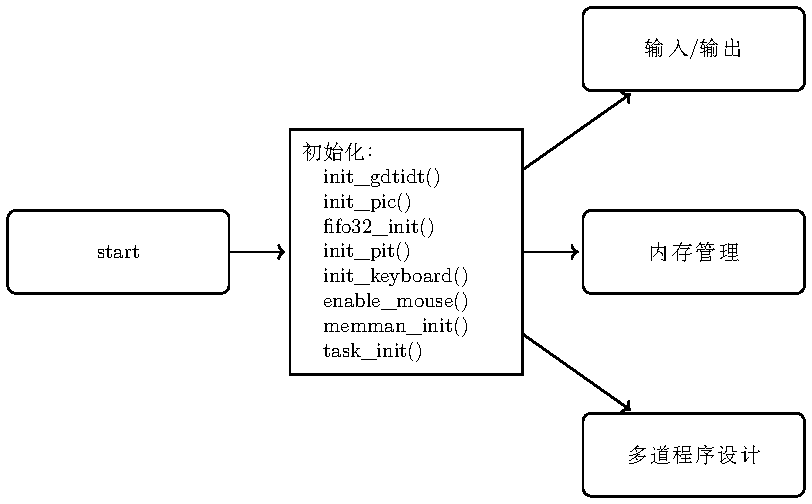
\includegraphics[width=.8\textwidth]{fig/func/run.pdf}
    \caption{全览}
    \label{fig:run}
  \end{figure}

\section{缓冲区}
\begin{figure}[H]
    \centering
    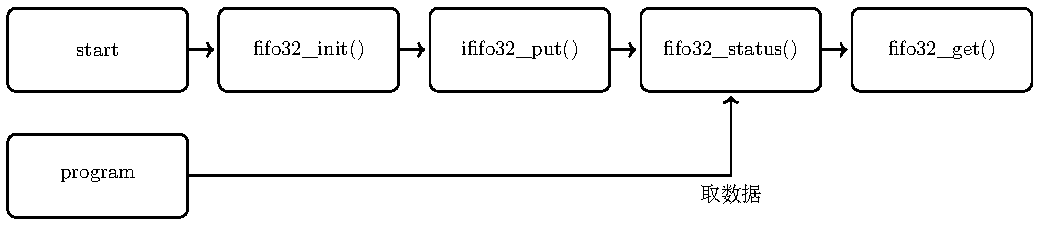
\includegraphics[width=.2\textwidth]{fig/func/fifo.pdf}
    \caption{缓冲区}
    \label{fig:fifo}
  \end{figure}

\section{内存管理}
\begin{figure}[H]
    \centering
    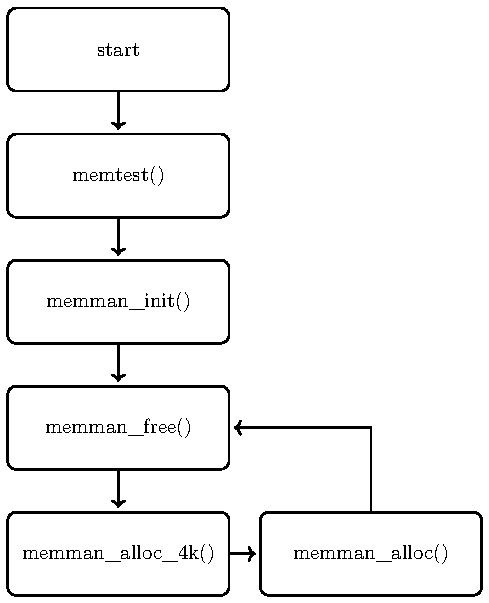
\includegraphics[width=.5\textwidth]{fig/func/memman.pdf}
    \caption{内存管理}
    \label{fig:memman}
  \end{figure}
  
  \section{输入输出}
\begin{figure}[H]
  \centering
  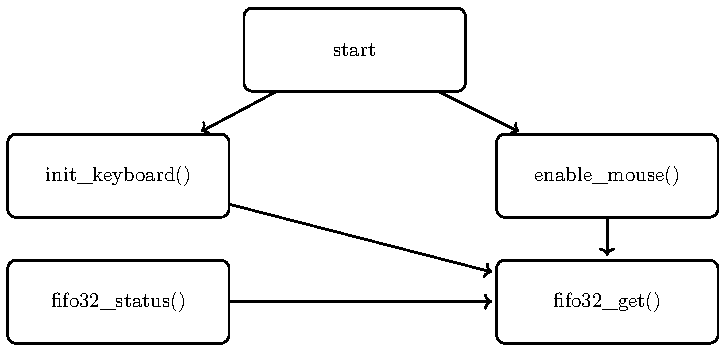
\includegraphics[width=.5\textwidth]{fig/func/io.pdf}
  \caption{输入输出}
  \label{fig:io}
\end{figure}

\section{多道程序设计及分时操作系统}
\begin{figure}[H]
  \centering
  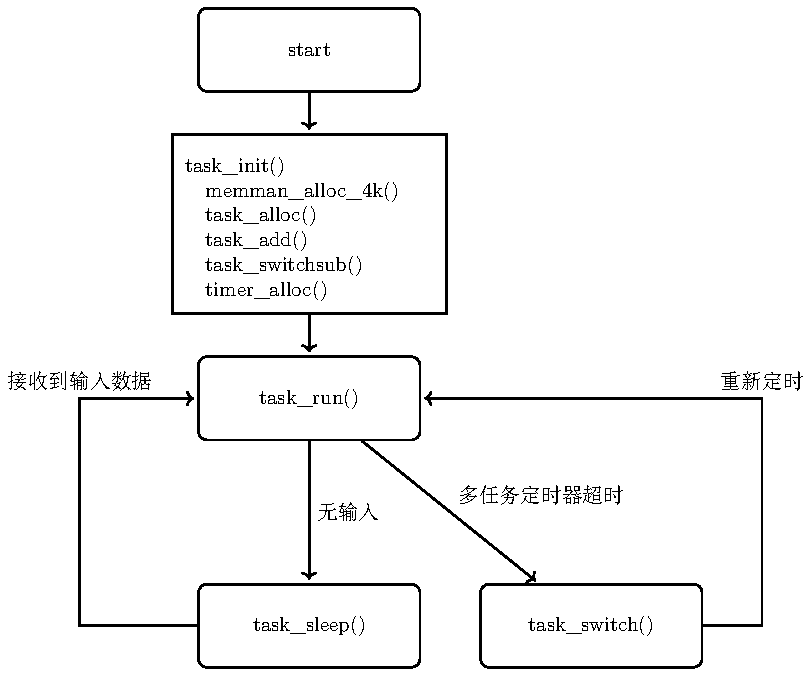
\includegraphics[width=.2\textwidth]{fig/func/multi.pdf}
  \caption{多道程序设计及分时操作系统}
  \label{fig:memman}
\end{figure}


